
%----------------------------------------------------------------------------------------
%	PACKAGES AND OTHER DOCUMENT CONFIGURATIONS
%----------------------------------------------------------------------------------------

\documentclass[twoside,twocolumn]{article}

\usepackage{blindtext} % Package to generate dummy text throughout this template 

\usepackage{amsmath}
\usepackage{graphicx}
\usepackage{mathrsfs}
\usepackage{subfig}
\usepackage{wrapfig}
\usepackage{listings}
\usepackage{float}

\usepackage[utf8]{inputenc}
\usepackage[sc]{mathpazo} % Use the Palatino font
\usepackage[T1]{fontenc} % Use 8-bit encoding that has 256 glyphs
\linespread{1.2} % Line spacing - Palatino needs more space between lines
\usepackage{microtype} % Slightly tweak font spacing for aesthetics
\usepackage{cite} %Citing references
\usepackage[english]{babel} % Language hyphenation and typographical rules

\usepackage[hmarginratio=1:1,top=32mm,columnsep=20pt]{geometry} % Document margins
%\usepackage[hang, small,labelfont=bf,up,textfont=it,up]{caption} % Custom captions under/above floats in tables or figures
%\usepackage{booktabs} % Horizontal rules in tables

\usepackage{lettrine} % The lettrine is the first enlarged letter at the beginning of the text

\usepackage{enumitem} % Customized lists
\setlist[itemize]{noitemsep} % Make itemize lists more compact


\usepackage{titlesec} % Allows customization of titles
\renewcommand\thesection{\Roman{section}} % Roman numerals for the sections
\renewcommand\thesubsection{\roman{subsection}} % roman numerals for subsections
\titleformat{\section}[block]{\large\scshape\centering}{\thesection.}{1em}{} % Change the look of the section titles
\titleformat{\subsection}[block]{\large}{\thesubsection.}{1em}{} % Change the look of the section titles

\usepackage{fancyhdr} % Headers and footers
\pagestyle{fancy} % All pages have headers and footers
\fancyhead{} % Blank out the default header
\fancyfoot{} % Blank out the default footer
\fancyhead[C]{Analytic model of cochlea} % Custom header text
\fancyhead[R]{\href{https://github.com/Kristopy/MoS2-Analysis}{GitHub}} % Custom header text
\fancyfoot[RO,LE]{\thepage} % Custom footer text

\usepackage{titling} % Customizing the title section

\usepackage{hyperref} % For hyperlinks in the PDF

%----------------------------------------------------------------------------------------
%					PICTURES-PATH
%----------------------------------------------------------------------------------------
\graphicspath{{Pictures/}} %Path to pictures

%----------------------------------------------------------------------------------------
%	TITLE SECTION
%----------------------------------------------------------------------------------------
\setlength{\droptitle}{-2\baselineskip} % Move the title up

\pretitle{\begin{center}\huge\bfseries} % Article title formatting
\posttitle{\end{center}} % Article title closing formatting
\title{Analytic model of cochlea}% Article title
\author{%
\normalsize{Written by}:\\	 	
\textsc{Kristoffer Varslott} \\\\
\normalsize {Department of Physics UiO}
}
\date{\today} % Leave empty to omit a date
\renewcommand{\maketitlehookd}




%----------------------------------------------------------------------------------------

\begin{document}

% Print the title
\maketitle

%----------------------------------------------------------------------------------------
%	ARTICLE CONTENTS
%----------------------------------------------------------------------------------------

%----------------------------------------------------------------------------------------------------------------
%     INTRODUTCTION
%----------------------------------------------------------------------------------------------------------------

\section{introduction}
\lettrine[nindent=0em,lines=2]{T}{his} article will consider the profound mechanical dynamics in the cochlea. Where we will look at where sound is perceived in cochlea. The interesting fact  that will come to place is the phenomena of vibrational resonance within the cochlea. We shall consider a range of input frequencies and where we have resonance in the cochlea. This article is based on the previous finding carried out by L.C Peterson and B.P. Bogert \cite{Peterson2005}. They were investigating the hydrodynamical theory in the cochlea, as how the basilar membrane was affected by a certain range of frequencies. An interesting fact stated in \cite{Zweig1976} was that Von Békésy found that basilar membrane traveled only in one direction, from the stapes towards the helicotrema. Waves traveling in both directions simultaneously would have given a more complicated pattern of displacement. So we will only look at waves propagating in one direction. 

\bigskip 

Cochlea consist of a three main parts, as illustrated in the figure. Scala vestibuli is on the top and consist of the fluid endolymph which similar to water \footnote{The viscosity of the endolymph is near that of water,  $n_e \approx 1 \cdot 10^{-2} cgs$ \cite{Zwislocki1980}}. This fluid is also in place at the bottom, which is called scala tympani. These to regions is separated by the basilar membrane, this membran is the key component in the analyses of the cochlea. For sound waves to enter the cochlea we need an input. This input is called the oval window. 

\begin{figure}[ht]
\centerline{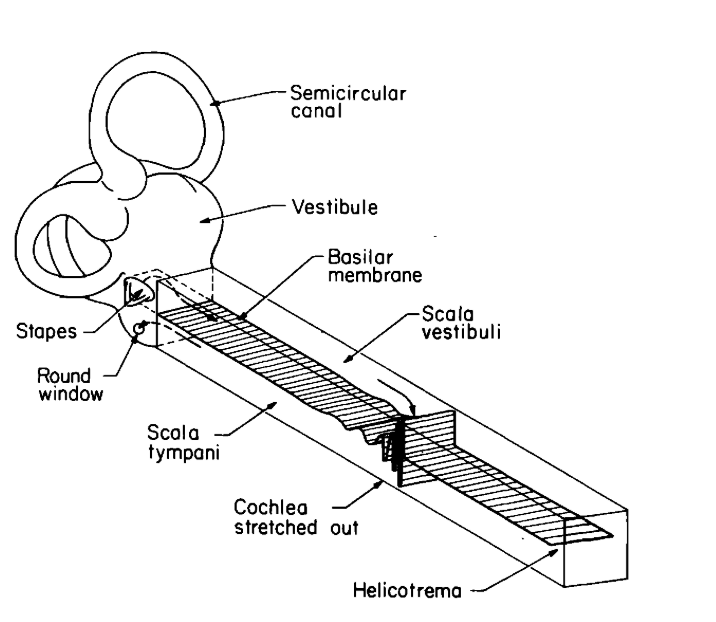
\includegraphics[scale= 0.60]{Pictures/cochlea.png}}
\caption{Simplified illustration of cochlea from \cite{Zweig1976}}
\end{figure}

\begin{figure*}[ht]
\centerline{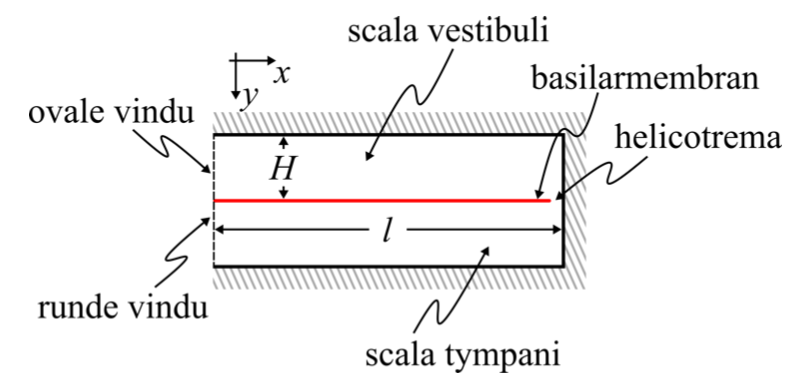
\includegraphics[scale= 0.75]{IllustrationCochlea.png}}
\caption{Simplified illustration of cochlea}
\end{figure*}


The stapes (stirrup) ossicle bone, placed outside the oval window transmitts a signal corresponding to the frequency of the sound input to the scala vestibuli. The stapes vibrations that is transformed into the cochlea is the range of frequencies we shall investigate. What is interesting is the fluctuating pressure difference between scala vestibuli and tympani across the basilarmebran. These pressure differences gives rise to the oscillation along basilar membrane, which we will take a closer look at. At the end of the cochlea we found an opening between the scala vestibuli and tympani. This opening is called helicotrema, and is vital for the dynamics within the cochlea. At this point we see no difference in pressure due to the opening. The pressure waves in scala vestibuli set in the x-direction, while the pressure waves in scala tympani is in the -x-direction. Our main task is to find at which point along the basilar membrane we see vibrational resonance. 

\bigskip

(Robles, Luis, Ruggero, Mario A) in Mechanics of the mammalian cochlea,  said that there is an general agreement that the energy delivered to the cochlea by the stapes  is transported principally via pressure waves in the cochlear fluids \cite{Robles2001}, as mentioned. As the fluid pressure interacts with the flexible basilar membrane. We shall look at how these waves varies within the cochlea as the pressure difference is decreasing towards the helicotrema. One interesting notion is how all of this is affected by resonance at certain location on the basilar membrane.

\bigskip 

The two dimensional model which we are constructing is discussed in a brilliant manner in Viergever, M A \cite{Viergever1977}. Where he solved the problem in an alternate way. He considered the complexity of the perilymph, and its compressibility. His results emphasizes the fact that the number of oscillators effect the resonance. 


%----------------------------------------------------------------------------------------------------------------
%                                         METHOD
%----------------------------------------------------------------------------------------------------------------

\section{method}
 
 
 To start off our consideration we need to look at the flux of mass through a small volum element between x and $x + \Delta x$. We take the mass density to be $\rho = 1 g/cm^3$, and the length of scala vestibuli to be $l = 3.5cm$ and the height $H = 0.67cm$. The mass flux through x from the left gives us: 
 
 \begin{equation}
 F(x) = \rho b H u(x)
 \end{equation}
 
 where b (constant) is the width, which we shall see, cancels out in the derivation to come. u(x) is the velocity in x-direction.
 
Further on we have that the mass flux out from the volum element can be written as: 

 \begin{equation}
 F(x + \Delta x) = \rho b H u(x + \Delta x)
 \end{equation}
 
 As we can see, the mass of the volume element increases as the flux of mass $F(x)$ on the left side enters and decreases as flux of mass $F(x + \Delta x)$ leaves the volume element. 
 
 The change of mass is therefore formulated as: 
 
\begin{equation}
\frac{\partial m(x)}{\partial t} = bH \Delta x \frac{\partial \rho}{\partial t} 
\end{equation}
 
\begin{equation}
bH \Delta x \frac{\partial \rho}{\partial t} = F(x) - F(x + \Delta x) - \rho b \Delta x \frac{\partial \eta}{\partial t}
\end{equation}
 
 We can approximate the last expression by Taylor series \footnote{$F(x + \Delta x) \approx F(x) + \partial F/\partial x \Delta x$}, and end up with: 
 
 \begin{equation}
bH \Delta x \frac{\partial \rho}{\partial t} = -\rho b H \frac{\partial u}{\partial x} \Delta x - \rho b \Delta x \frac{\partial \eta}{\partial t}
\end{equation}

 \begin{equation}
H\frac{\partial \rho}{\partial t} = -\rho H \frac{\partial u}{\partial x}  - \rho \frac{\partial \eta}{\partial t}
\end{equation}
 
 
 Now we have introduced a new parameter $\eta$, this is the amplitude of the basilar membrane. As we can see it is gives as the time derivative. Also both $\Delta x$ and the width b cancels out.  Further on we need a way to express the pressure within the scala vestibuli. We introduce: 
 
 \begin{equation}
c^2 \frac{\partial \rho}{t} = \frac{\partial p}{\partial t}
\end{equation}

Inserting this into the expression for change of mass yields: 

 \begin{equation}\label{eq:1}
\frac{H}{c^2}\frac{\partial p}{\partial t} = -\rho H \frac{\partial u}{\partial x}  - \rho \frac{\partial \eta}{\partial t}
\end{equation}

These calculation can also be done on scala tympani which gives us: 

 \begin{equation}\label{eq:2}
\frac{H}{c^2}\frac{\partial q}{\partial t} = -\rho H \frac{\partial v}{\partial x}  + \rho \frac{\partial \eta}{\partial t}
\end{equation}
 
 Where q and v is the pressure and velocity in scala tympani. As mentioned earlier the stapes vibrates according to the sound input. These vibrations is transformed into pressure waves within the cochlea (scala vesitbuli). The pressure differences along the x-axis gives rise to acceleration. This can be expressed as: 

Scala Vesitbali: 
\begin{equation}\label{eq:3}
\rho\frac{\partial u}{\partial t} = -\frac{\partial p}{\partial x} 
\end{equation}

Scala tympani:
\begin{equation}\label{eq:4}
\rho\frac{\partial v}{\partial t} = -\frac{\partial q}{\partial x} 
\end{equation}

If we go back to the basilar membrane, we can form a model consisting of a number of harmonic oscillators with an amplitude $\eta$, which are moves due to the pressure difference (p-q): 
\begin{equation}
m\frac{\partial^2\eta}{\partial t^2} + k\eta = p-q = \xi
\end{equation}

Where $\xi$ is the pressure difference between the pressure formed in scala vestibuli and tympani and k is the stiffness of the membrane along x. This is decreasing with x: k = $4\times10^9 e^{-4x}g/cm^2s^2$

\bigskip

We will now build a model of the cochlea by using these equations. By this we would like to find a wave equation which describes the basilar membrane oscillation across the length $l$. Firstly we want to discriminate the velocities u(x) and v(x) from equation (\ref{eq:1}) and (\ref{eq:2}). We may do this by using (\ref{eq:3}) and (\ref{eq:4}). By taking the second derivative of these equation and substituting. 
\bigskip

 \begin{equation}
\frac{H}{c^2}\frac{\partial p}{\partial t} = -\rho H \frac{\partial u}{\partial x}  - \rho \frac{\partial \eta}{\partial t}
\end{equation}

\begin{equation}
\rho\frac{\partial u}{\partial t} = -\frac{\partial p}{\partial x} 
\end{equation}

And then taking the second derivative with respect to x and t: 

 \begin{equation}
    \left\{
                \begin{array}{ll}
                  \frac{H}{c^2}\frac{\partial^2 p}{\partial t^2} = -\rho H \frac{\partial^2 u}{\partial x\partial t}  - \rho \frac{\partial^2 \eta}{\partial t^2}\\
                  \\
                 \frac{H}{c^2}\frac{\partial^2 p}{\partial t \partial x} = -\rho H \frac{\partial^2 u}{\partial x^2}  - \rho \frac{\partial^2 \eta}{\partial t\partial x}
                \end{array}
              \right.
\end{equation}

\bigskip

 \begin{equation}
    \left\{
                \begin{array}{ll}
                  \rho\frac{\partial^2 u}{\partial t^2} = -\frac{\partial^2 p}{\partial x\partial t}\\
                  \\
                  \rho\frac{\partial^2 u}{\partial t\partial x} = -\frac{\partial^2 p}{\partial x^2}
                \end{array}
              \right.
\end{equation}

\bigskip

As we can see, that it is possible to substitute $ \rho\frac{\partial^2 u}{\partial t\partial x}$. By this we have managed to discriminate the velocity u(x) in scala vestibuli. The result yields: 

 \begin{equation}
 \frac{H}{c^2}\frac{\partial^2 p}{\partial t^2} = H \frac{\partial^2 p}{\partial x^2}  - \rho \frac{\partial^2 \eta}{\partial t^2}
\end{equation}

Doing the same for scala tympani gives us: 

 \begin{equation}
 \frac{H}{c^2}\frac{\partial^2 q}{\partial t^2} = H \frac{\partial^2 q}{\partial x^2}  + \rho \frac{\partial^2 \eta}{\partial t^2}
\end{equation}

Now we need to reintroduce the pressure difference $\xi$ to be able to build the model. Our new expressions have both pressures (p and q), but the second derivatives.  We know from earlier that: 

 \begin{equation}
\xi = p - q
\end{equation}

By this we may reorder our expression to give the second derivatives of p and q with respect to x on one side: 

 \begin{equation}\label{eq:5}
\frac{\partial^2 p}{\partial x^2} =  \frac{1}{c^2}\frac{\partial^2 p}{\partial t^2}    + \frac{\rho}{H} \frac{\partial^2 \eta}{\partial t^2}
\end{equation}

 \begin{equation}\label{eq:6}
\frac{\partial^2 q}{\partial x^2} =  \frac{1}{c^2}\frac{\partial^2 q}{\partial t^2}    - \frac{\rho}{H} \frac{\partial^2 \eta}{\partial t^2}
\end{equation}

Inserting in $\xi = p - q$ gives: 

 \begin{equation}
\frac{\partial^2 \xi}{\partial x^2} = \frac{\partial^2 p}{\partial x^2} - \frac{\partial^2 q}{\partial x^2} 
\end{equation}

Further we can see that the last term of \ref{eq:5} and \ref{eq:6}, and we end up with: 

 \begin{equation}
\frac{\partial^2 \xi}{\partial x^2} = \frac{1}{c^2}\left [\frac{\partial^2 p}{\partial t^2} -\frac{\partial^2 q}{\partial t^2} \right] +  \frac{2\rho}{H} \frac{\partial^2 \eta}{\partial t^2}
\end{equation}

which can further be rewritten as: 

 \begin{equation}
\frac{\partial^2 \xi}{\partial x^2} = \frac{1}{c^2} \frac{\partial^2 \xi}{\partial t^2} +  \frac{2\rho}{H} \frac{\partial^2 \eta}{\partial t^2}
\end{equation}

 \begin{equation}
\frac{\partial^2 \xi}{\partial t^2}  = c^2\frac{\partial^2 \xi}{\partial x^2} +  \frac{2\rho c^2}{H} \frac{\partial^2 \eta}{\partial t^2}
\end{equation}


This is our result, and it is in the form of a wave equation with the extra part consisting of the second derivative of $\eta$. This expression describes the dynamics of pressure difference. 


Now we need to make  a discrete evaluation of the equations. We are left with two equations which is sufficient for modeling the cochlea system. 

 \begin{equation}\label{eq:7}
\frac{\partial^2 \xi}{\partial t^2}  = c^2\frac{\partial^2 \xi}{\partial x^2} -  \frac{2\rho c^2}{H} \frac{\partial^2 \eta}{\partial t^2}
\end{equation}

\begin{equation}\label{eq:8}
m\frac{\partial^2\eta}{\partial t^2} + k\eta = p-q = \xi
\end{equation}

We need to find a numerical approach to these differential equations. First we name our variables x and t for i and j. Which will help us indexing. 


\begin{equation}
\xi(x,t) = \xi(x_i,t_j) \equiv \xi_{i,j}  
\end{equation}
\begin{equation}
\eta(x,t) = \eta(x_i,t_j) \equiv \eta_{i,j}  
\end{equation}

Also by taking a numerical approach towards the derivatives find a way to calculate for the next step, in time and position. We will show it using $\xi$: 

 \begin{equation}
\frac{\partial^2 \xi}{\partial x^2}  = \xi_{xx,i,j} = \frac{\xi_{i+1,j} - 2\xi_{i,j} + \xi_{i-1,j}}{\Delta x^2}
\end{equation}

\begin{equation}
\frac{\partial^2 \xi}{\partial t^2}  = \xi_{tt,i,j} = \frac{\xi_{i,j + 1} - 2\xi_{i,j} + \xi_{i,j-1}}{\Delta t^2}
\end{equation}

On this note equation (\ref{eq:7}) may be written more compactly as: 


 \begin{equation}\label{eq:9}
\xi_{tt,i,j}   = c^2 \xi_{xx,i,j} +  \frac{2\rho c^2}{H} \eta_{tt,i,j}
\end{equation}

Solving $\xi_{i,j+1}$, the next timestep for the pressure difference instance: 


\begin{multline*}
\xi_{i,j+1} = \left(c\frac{\Delta t}{\Delta x}\right)^2\left( \xi_{i+1,j} - 2\xi_{i,j} + \xi_{i-1,j} \right)  \\ 
- \frac{2\rho c^2 \Delta t^2}{Hm} \left(\xi_{i,j} - k\eta_{i,j}\right) + 2\xi_{i,j} -\xi_{i,j-1}
\end{multline*}

We have arrived at this equation by rewriting equation (\ref{eq:8}) by numerical method: 

\begin{equation}
\frac{\partial^2\eta}{\partial t^2}  = \frac{ \left(\xi -  k\eta \right)}{m}
\end{equation}

\begin{equation}
\eta_{tt,i,j} = \frac{ \left(\xi_{i,j} -  k\eta_{i,j} \right)}{m}
\end{equation}

For then to insert this back into equation (\ref{eq:9}). We can also figure out the next time step for $\eta_{tt,i,j}$: 
\begin{equation}
\eta_{i,j + 1} = \frac{\Delta t^2}{m}\left(\xi_{i,j} - k\eta_{i,j}\right) + \eta_{i,j} - \eta_{i,j-1}
\end{equation}

These equations can be written more compactly if we define som variables and reorder: 

\begin{equation}
C =  c\frac{\Delta t}{\Delta x}
\end{equation}

\begin{equation}
\alpha = \frac{2\rho}{H}
\end{equation}

\begin{equation}
\beta =  \frac{\Delta t^2}{m}
\end{equation}

\begin{multline*}
\xi_{i,j+1} =C^2\left(\xi_{i+1,j} -2\xi_{i,j} + \xi_{i-1,j}\right) + 2\xi_{i,j} \\
-\xi_{i,j-1} - \alpha\left(\eta_{i,j+1} -2\eta_{i,j} + \eta_{i,j-1}\right)
\end{multline*}

\begin{equation}
\eta_{i,j + 1} = \beta \left( \xi_{i,j}- k\eta_{i,j}\right) + 2\eta_{i,j} - \eta_{i,j-1}
\end{equation}


We have know figured out an analytic approach to our problem. The next step is to evaluate the boundary conditions and also consider the Courant condition. First off we know that the pressure difference $\xi_{l, t} = 0$, because of the helicotrema. And at position zero we need an initial force to initiate our model.This force comes from the stapes that vibrates with a frequency \cite{Robles2001}. We set this condition to be $ \xi_{0, t} = Asin(\omega \cdot t)$, where A is the amplitude of 60dB which converts into 0.2Pa. $\omega$  possesses the frequency at which the stapes vibrates.

\bigskip

 Now we have found the initial conditions for for the pressure difference at position zero and at the end of the basilar membrane. We need to investigate the Courant condition, which is the C that we defined earlier. This C must fulfill the condition C < $C_{max}$, where $C_{max}$ usually lies at 1, but for our problem we are investigating a wave equation which gives us a Courant condition half of this. Which means it should lie at 0.5. For this to be the case we need to find appropriative $\Delta x$ and $\Delta t$.
 
 Implementing these conditions to our script and looking at max values of $\eta$ at different times, we will see a plot over the resonance at a certain location at the basilar membrane. 

Using parameters as, $m = 0.143g/cm^2$, $c = 1.43 \times 10^5 cm/s$

%----------------------------------------------------------------------------------------------------------------
%                                                  RESULTS
%----------------------------------------------------------------------------------------------------------------

\section{numerical results}

A numerical program has been developed, and our goal here is to look at our result. By looking at different frequencies at the stapes we were able to see different resonances occurring at certain locations in the basilar membrane. We will look at frequencies at f = [500Hz, 2kHz, 5kHz, 10kHz].

\subsection{What is to be expected?}

\begin{figure*}[ht]
\centerline{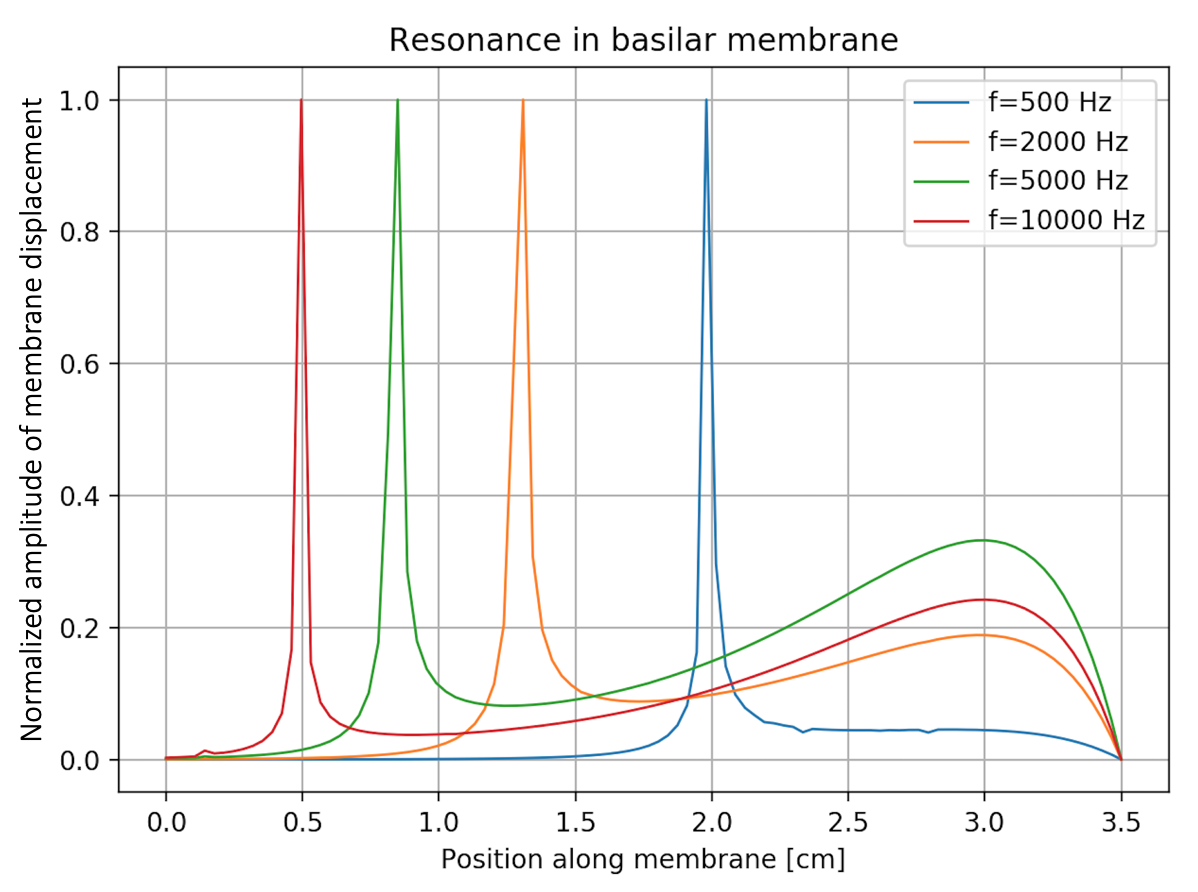
\includegraphics[scale= 0.55]{CorrectResonance.png}}
\caption{High precision plot of resonance frequencies for f = [500, 2000, 5000, 10000]Hz \\ High precision along membrane, with normalized amplitude}
\end{figure*}

 What we experienced was that the resonance is dependent on a number of different parameters. In the analytic approach we figured out the boundary conditions and also the force which initiated our system. What was interesting in our program was that small adjustment to the time and number of oscillators effected our result a great deal. 
 
Theory suggest that high frequency resonance should occur close to the oval window, while low frequency resonance should occur close to the helicotrema. While our model try to interpret the real cochlea Our computing power falls short, it is simply not good enough to simulate a better approximation off cochlea. 
 
\bigskip



%The amplitude of the basilar membrane is also one thing to anticipate to change with various frequencies. We are going to look at the resonance locations, but at what amplitude does these resonances have, and are they changing with input frequencies? If we recall that k = $4\times10^9 e^{-4x}g/cm^2s^2$, we may anticipate an increasing amplitude as the resonances occur throughout the membrane. 


\subsection{Results}


Figure 3 shown below is a plot over various frequency input, which responds within the cochlea. What we see here is the resonance at f = [500Hz, 2kHz, 5kHz, 10kHz]. 
As we can see, the precision in position along the membrane is rather high, we get clear peaks at certain points along x-axis. In our program we used various N = 100. With time set to 0.2s.  There were a lot of calculations within the certainty at the locations. Of course N = 100 oscillators is not ideal, at all, but we were able to see som good results after all.

\bigskip
The systems natural frequencies can be calculated, and thereby controlling where resonance will occure. By calculating this for the range of frequencies in which we where had resonance we will see if our model checks out. We have that natural frequency $\omega_0 = \sqrt{\frac{k}{m}}$ and thereby our systems frequency at the x position we had resonance: 

\begin{equation} 
f_{f.res} = \frac{1}{2\pi}\sqrt{\frac{4 \times 10^9 e^{-4x}}{m}}
\end{equation}

Gives us $ f_{f.res}(x = 2cm) \approx 500Hz$, this fits nicely and for all the others we have:  $ f_{f.res}(x = 1.3cm) \approx 2000Hz $,  $ f_{f.res}(x = 0.8cm)\approx5000Hz $ and  $ f_{f.res}(x = 0.5cm) \approx 10000Hz $. This approximation tells us we are on the right way. 

\bigskip

The human cochlea possesses around 3500 oscillators. As we see in figure 3, resonance occures at at all frequencies as expected, also the highest frequencies takes place closest to the oval window while lower frequencies goes toward helicotrema. 

\bigskip

The reason for our choice of time is cleared out in figure 4. Where we see the variation of resonance with time. We have here plotted for frequency 500 Hz. This corresponds to a period of T = 1/f = 2ms. At this time we have the minimum precision. As we increase the time we see that some sort of sharper peak starts to appear, at the time 0.2s, we see the clear peak that appeared in figure 3.  



\begin{figure}[ht]
\centerline{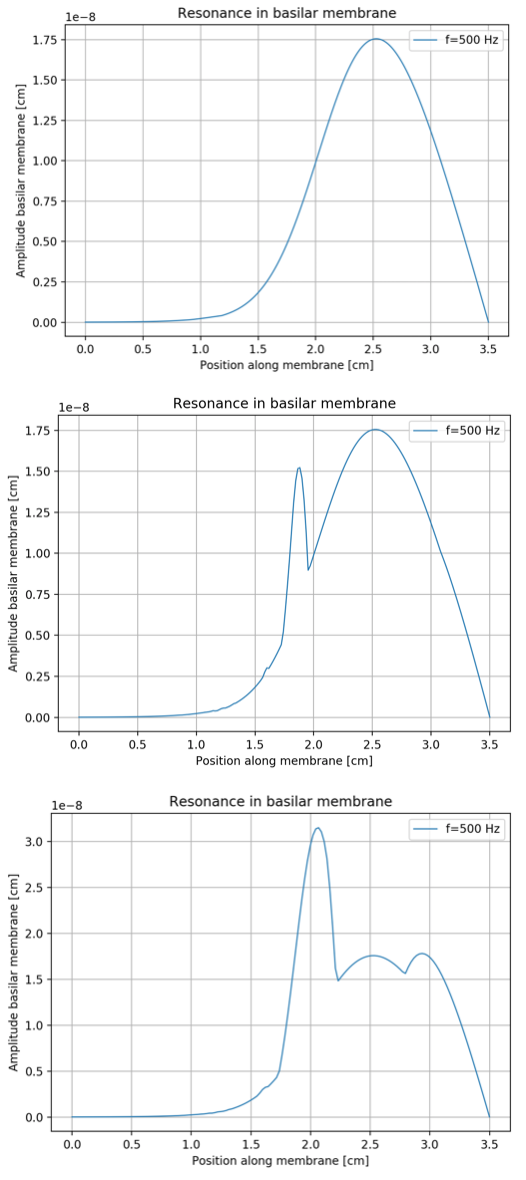
\includegraphics[scale= 0.65]{Pictures/together.png}}
\caption{At different times for f = 500Hz \\ t = [0.002, 0.0025,0.0034]s, }
\end{figure}

\bigskip
Figure 3 is plotted with normalized amplitude of displacement due to large differences for various frequencies.  Another interesting thing about figure 3 is the bulks appearing for 2, 3, 10 kHz frequencies. Which does not represent any resonance. 

\bigskip

Figure 5 showes the displacement in basilar membrane at M-1. This plot is interesting because it tells us how the membrane vibrates along the membrane, for time set at 2ms. This time was as explained to be the minimum. We clearly see that it is hard to determine where resonance takes place. In figure 3 we see no such bulk appearing, this is due to the choice of time. While satisfying the conditions for one frequency, it affects the condition for the other.  

\begin{figure}[ht]
\centerline{\includegraphics[scale= 0.45]{Pictures/displacement.png}}
\caption{Plot of $\eta(x,t_{M-1})$, f = 500Hz for  t = [0.002]s, N = 50. Great uncertainty in where the resonance is occuring}
\end{figure}

\begin{figure}[ht]
\centerline{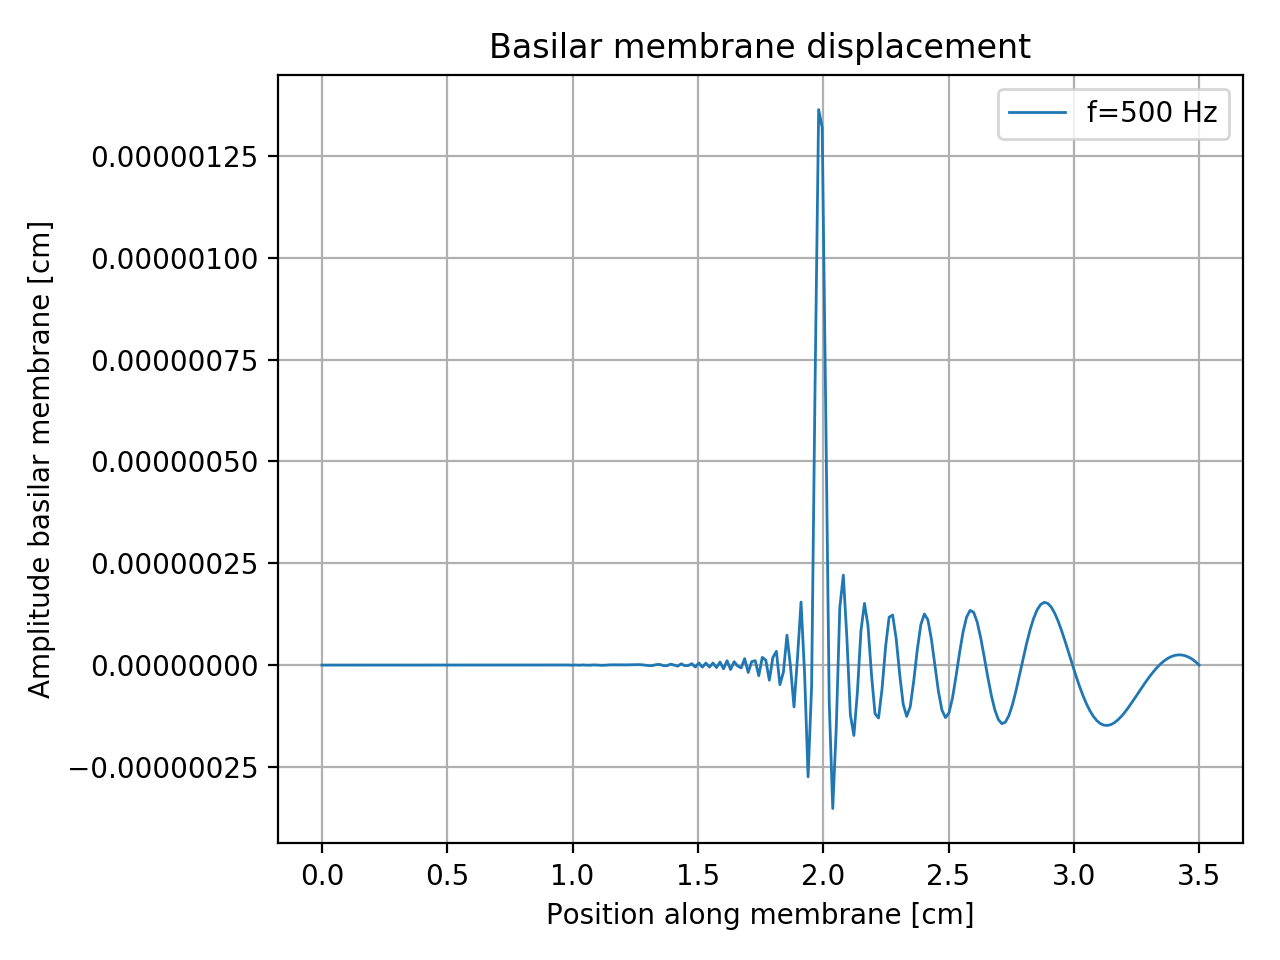
\includegraphics[scale= 0.45]{Pictures/N250s0015.png}}
\caption{Plot of $\eta(x,t_{M-1})$, f = 500Hz for  t = [0.015]s, N = 250. Less uncertainty }
\end{figure}


Figure 6 shows us where the displacement of basilar membrane takes place. Along with other propagating waves after the resonance. Ideally we should have computed with larger N and larger t- value. We can see in figure 5 and 6, that there is a large difference in certainty for chancages in number of oscillators and time. 
%----------------------------------------------------------------------------------------------------------------
%                                                DISCUSION
%----------------------------------------------------------------------------------------------------------------

\bigskip

\section{discusion}

These results need to be dissected. The profound difficulty lies in the uncertainty of resonance occurrence.  As seen in the results, our peaks appeared at different locations depending on the time we set, and number of oscillators. Figure 3, shows som great plots, where it seems as we have got some sharp peaks indicating with great certainty where the resonance is. What is interesting by this plot is the bulks appearing in the higher frequencies. 

\bigskip

As mentioned, the time for this plot was 0.2s. This time should be more than enough to cover the 500Hz frequency with high certainty.  As we see 500Hz is almost flat after the resonance. While the other frequencies show some uncertainty. It is hard to explain exactly what is going on here, according to theory the wave should have died out relatively fast after the resonance, so we should not get any $peak$, after resonance. 

\bigskip

Of course the height of the bulk at f = 500Hz in figure 3 relative to the others is low, but we still have some uncertainty. We still need to remember that this is just a model, and that our model does not consider a lot of details that may be vital for absolutely correct results f.ex damping. By implementation damping of the pressure wave within cochlea would  probably give a more realistic result. Also by considering height differences along x-axis [H(x)], would be more realistic, as L.C Peterson and B.P Bogert does \cite{Peterson2005} . 

 \bigskip

Figure 4, shows as mentioned maximum amplitude of basilar membrane along x-axis. Here we clearly see what is happening as we increase the time for minimum time, set as period time at the given frequency. As we increase the time, some sort of wave starts to propagate through the sample, and we are left with a sharp peak. What is interesting to note, is that this does not occure if we use cosine instead of sinus in the pressure force term. This is peculiar, as a sinusoidal function is our preferred and natural choice due to its starting point at zero. 


%----------------------------------------------------------------------------------------------------------------
%                                               CONCLUSION
%----------------------------------------------------------------------------------------------------------------

\section{conclusion}


To conclude this article we may look at our model, which served it purpose by producing some qualitatively good data. Our method, gave us a fine approximation in the program. By using an analytic approach and making a discrete evaluation of the partial differential equation, we where able to make a formula that calculate the next time step. By looking at our problem with ease, we could solve the initial conditions, which simply was zero, except of our initial force.  

\bigskip

Our plot gave som fine values, but abnormalities where present, as discussed earlier. We found out where resonance took place within the cochlea at high precision, and also the importance of time duration and number of oscillations to get a valid result. \cite{Inselberg2005}

%----------------------------------------------------------------------------------------
%	REFERENCE LIST
%----------------------------------------------------------------------------------------

\onecolumn
\bibliographystyle{unsrt}
\bibliography{BiBTeX/ProjectAssignmentFYS2130.bib}

%----------------------------------------------------------------------------------------

\end{document}
